% ================================================================
\chapter{Tabelas hash}\label{cap:hash}\label{sec:hash}
% ================================================================
\begin{objetivos}
\begin{itemize}
  \item Dicionários, endereçamento direto e a ideia de uma função hash.
  \item Funções hash clássicas e o problema inevitável das colisões.
  \item Tratamento de colisões por encadeamento e por endereçamento aberto.
  \item A complexidade em função do fator de carga, e quando preferir uma tabela hash a uma árvore de busca.
\end{itemize}
\end{objetivos}

Um \textbf{dicionário} guarda pares (chave, valor) e oferece inserção, busca e remoção por chave. As árvores AVL do Capítulo~\ref{cap:avl} implementam dicionários com todas as operações em $O(\log n)$ e ainda mantêm as chaves em ordem. Quando a ordem não importa, é possível fazer melhor: as \textbf{tabelas hash} transformam a chave diretamente num endereço e realizam as operações em tempo $O(1)$ esperado.

\section{Endereçamento direto e funções hash}
Se as chaves são inteiros de um universo pequeno $U=\{0,\dots,M-1\}$, basta um vetor de tamanho $M$ indexado pela própria chave: é o \textbf{endereçamento direto}, com todas as operações em $O(1)$. Mas o universo de chaves costuma ser enorme ou infinito (todos os inteiros de 64 bits, todas as strings), e a memória é finita. Uma \textbf{função hash} $h:U\to\{0,\dots,m-1\}$ transforma cada chave num endereço de uma tabela de $m$ posições, com $m$ da ordem do número de chaves efetivamente guardadas.

\begin{exemplo}[Do endereçamento direto à função hash]\label{ex:enddireto}
Uma turma tem alunos com matrículas de 0 a 9, e estão presentes os de matrícula 2, 5 e 7. Com endereçamento direto, um vetor de 10 posições guarda cada aluno na posição da sua matrícula, e ``o aluno 5 está presente?'' é uma única consulta (Figura~\ref{fig:hashideia}). Se as matrículas fossem números de 9 dígitos, o vetor teria $10^9$ posições para guardar 3 alunos. Uma função hash, como $h(k)=k\bmod 7$, comprime o universo: as matrículas $201\,345\,002$, $731\,000\,006$ e $555\,777\,016$ vão para os endereços 5, 2 e 4 de uma tabela com 7 posições.
\begin{figura}[À esquerda, endereçamento direto: a chave é o próprio endereço. À direita, uma função hash leva chaves de um universo enorme a uma tabela pequena.\label{fig:hashideia}]
\small
\begin{tabular}{@{}c@{\hspace{8mm}}c@{}}
\vetorz[2,5,7]{-,-,2,-,-,5,-,7,-,-} &
\begin{tikzpicture}[baseline=-0.6ex, x=10mm]
\foreach \pos/\val in {0/{},1/{},2/{\tiny\ldots006},3/{},4/{\tiny\ldots016},5/{\tiny\ldots002},6/{}} {
  \node[cel, minimum width=10mm] (t\pos) at (\pos,0) {\val}; \node[idx] at (\pos,0.48) {\pos};}
\end{tikzpicture}\\[2pt]
\scriptsize vetor de 10 posições & \scriptsize tabela de 7 posições, $h(k)=k\bmod7$
\end{tabular}
\end{figura}
\end{exemplo}

\paragraph{Funções clássicas.}
\begin{itemize}
  \item \emph{Divisão}: $h(k)=k\bmod m$, com $m$ primo e longe de potências de 2, para que o resultado dependa de todos os bits da chave.
  \item \emph{Multiplicação}: $h(k)=\floor{m\,(kA\bmod1)}$, com uma constante $0<A<1$; um valor muito usado é $A\approx(\sqrt5-1)/2$. Aqui o valor de $m$ é pouco crítico, e pode ser uma potência de 2.
  \item \emph{Dobra} e \emph{meio do quadrado}: combinam partes da chave, ou extraem os dígitos centrais de $k^2$.
  \item Para \emph{strings}, a função polinomial $h(s)=\big(\sum_is_i\,b^{i}\big)\bmod m$, calculada pela regra de Horner.
  \item \emph{Hashing universal}: a função é sorteada, no início, de uma família, como $h_{a,b}(k)=((ak+b)\bmod p)\bmod m$ com $p$ primo. Isso garante bom desempenho esperado para \emph{qualquer} conjunto de chaves, sem depender de a entrada ser ``aleatória''.
\end{itemize}

\begin{exemplo}[Calculando endereços]
\textbf{Divisão}, com $m=13$: $h(100)=100\bmod13=9$ e $h(2026)=2026\bmod13=11$.
\textbf{Multiplicação}, com $m=16$ e $A=0{,}6180339887$: $100A\approx61{,}8034$, cuja parte fracionária é $0{,}8034$, e $h(100)=\floor{16\cdot0{,}8034}=12$; já $101A\approx62{,}4214$, e $h(101)=\floor{16\cdot0{,}4214}=6$. Chaves vizinhas caem em endereços distantes.
\textbf{String}, com as letras valendo $\mathtt a=1,\dots,\mathtt z=26$, $b=31$ e $m=97$: para ``gato'' (7, 1, 20, 15), a regra de Horner faz $h:=7$; $h:=(7\cdot31+1)\bmod97=24$; $h:=(24\cdot31+20)\bmod97=85$; $h:=(85\cdot31+15)\bmod97=31$. Em cada passo, $h$ fica menor que $m$, e nunca é preciso calcular $31^3$.
\textbf{Universal}, com $p=17$ e $m=6$: com $(a,b)=(3,4)$, as chaves 5 e 9 colidem, pois $((3\cdot5+4)\bmod17)\bmod6=2$ e $((3\cdot9+4)\bmod17)\bmod6=2$; com $(a,b)=(5,1)$, elas vão para os endereços 3 e 0. Um adversário que não sabe qual função foi sorteada não consegue escolher chaves que colidam sempre.
\end{exemplo}

\section{Colisões}
Uma \textbf{colisão} ocorre quando duas chaves diferentes recebem o mesmo endereço: $h(k_1)=h(k_2)$ com $k_1\ne k_2$. Colisões são inevitáveis, pelo princípio da casa dos pombos, pois $|U|>m$. E elas aparecem muito antes de a tabela ficar cheia: é o ``paradoxo do aniversário'', pelo qual, numa turma de apenas 23 pessoas, a chance de duas fazerem aniversário no mesmo dia (365 ``endereços'') já passa de 50\%. Há duas famílias de soluções.

\paragraph{Encadeamento.} No \textbf{encadeamento exterior}, cada posição da tabela aponta para uma lista com as chaves que receberam aquele endereço. Inserir é colocar a chave no início da lista, em $O(1)$; buscar e remover percorrem a lista. No \textbf{encadeamento interior}, as listas são formadas dentro da própria tabela, usando uma área de colisões ou ligando posições livres por ponteiros.

\begin{exemplo}[Encadeamento exterior]
Inserimos $12,44,13,88,23,94,11,39,20,16,5$, nessa ordem, numa tabela de $m=11$ posições com $h(k)=k\bmod11$ (Figura~\ref{fig:encadeamento}). As chaves 44, 88 e 11 vão todas para o endereço 0, e como cada uma entra no início da lista, ela fica $11\to88\to44$. Buscar 44 percorre a lista inteira (3 comparações); buscar 33, que também iria para o endereço 0, faz 3 comparações e conclui que a chave não está lá. Buscar uma chave de endereço 3 não faz nenhuma comparação: a lista está vazia.
\begin{figura}[Encadeamento exterior com $m=11$. Cada posição aponta para a lista das chaves que receberam aquele endereço; as inserções são feitas no início da lista.\label{fig:encadeamento}]
\begin{tikzpicture}[x=1cm,y=-0.62cm, no/.style={draw, thick, minimum width=8mm, minimum height=4.6mm, font=\scriptsize, inner sep=1pt, fill=white}]
\foreach \pos in {0,...,10} {\node[cel, minimum width=8mm, minimum height=5.2mm, fill=azul] (s\pos) at (0,\pos) {\pos};}
\foreach \pos/\lista in {0/{11,88,44},1/{23,12},2/{13},5/{5,16},6/{39,94},9/{20}} {
  \foreach \val [count=\k] in \lista {\node[no] (l\pos-\k) at (\k*1.3+0.3,\pos) {\val};}
  \draw[seta] (s\pos.east) -- (l\pos-1.west);
  \foreach \val [count=\k, evaluate=\k as \prox using int(\k+1)] in \lista {\ifnum\k>1 \pgfmathtruncatemacro{\ant}{\k-1}\draw[seta] (l\pos-\ant.east) -- (l\pos-\k.west); \fi}}
\end{tikzpicture}
\end{figura}
\end{exemplo}

\paragraph{Endereçamento aberto.} Todas as chaves ficam na própria tabela. Em caso de colisão, examina-se uma sequência de posições, chamada sequência de \emph{sondagem}, até encontrar uma livre:
\begin{itemize}
  \item \emph{sondagem linear}: $h(k,i)=(h(k)+i)\bmod m$, simples, mas sujeita a \textbf{agrupamento primário}: longas sequências de posições ocupadas, que tendem a crescer;
  \item \emph{sondagem quadrática}: $h(k,i)=(h(k)+c_1i+c_2i^2)\bmod m$, que reduz o agrupamento;
  \item \emph{duplo hashing}: $h(k,i)=(h_1(k)+i\,h_2(k))\bmod m$, com $h_2(k)$ primo com $m$, para que a sequência visite todas as posições.
\end{itemize}
No endereçamento aberto, uma remoção não pode simplesmente esvaziar a posição, pois isso interromperia as sequências de sondagem de outras chaves; a posição é marcada como ``removida''.

\begin{exemplo}[Sondagem linear e agrupamento]\label{ex:linear}
Inserimos $18,41,22,44,59,32,31,73$, nessa ordem, numa tabela de $m=13$ posições com $h(k)=k\bmod13$ e sondagem linear (Figura~\ref{fig:sondagem}). As chaves 18, 41, 22 e 59 vão direto para os endereços 5, 2, 9 e 7. O 44 tem $h=5$, ocupado pelo 18, e vai para 6 (2 sondagens). O 32 tem $h=6$: as posições 6 e 7 estão ocupadas, e ele vai para 8 (3 sondagens). O 31 tem $h=5$ e só encontra lugar na posição 10, depois de 6 sondagens; o 73, de $h=8$, vai para 11, com 4. As chaves formam um \textbf{agrupamento} contínuo das posições 5 a 11, e qualquer chave cujo endereço caia nesse trecho vai parar no seu fim, aumentando-o ainda mais.

Se outras funções de sondagem fossem usadas, a chave 31 seguiria outro caminho: com a sondagem quadrática $h(k,i)=(h(k)+i^2)\bmod13$, a sequência seria $5,6,9,1,\dots$; com o duplo hashing de $h_2(k)=1+(k\bmod11)=10$, seria $5,2,12,9,6,3,\dots$ --- saltos que espalham as tentativas e evitam o agrupamento.
\begin{figura}[Sondagem linear com $m=13$ depois das oito inserções do Exemplo~\ref{ex:linear}. O número abaixo de cada chave é a quantidade de sondagens que a sua inserção fez; as posições 5 a 11 formam um agrupamento.\label{fig:sondagem}]
\begin{tikzpicture}[x=8mm,y=7mm]
\fill[destaque] (4.5,-0.3) rectangle (11.5,0.3);
\foreach \val [count=\k from 0] in {{},{},41,{},{},18,44,59,32,22,31,73,{}} {\node[cel, minimum width=8mm] at (\k,0) {\val}; \node[idx] at (\k,0.55) {\k};}
\foreach \pos/\sd in {2/1,5/1,6/2,7/1,8/3,9/1,10/6,11/4} {\node[font=\tiny, text=BrickRed] at (\pos,-0.6) {\sd};}
\draw[seta, BrickRed!70, bend left=40] (5,0.85) to node[above, font=\tiny] {31: 5, 6, 7, 8, 9, 10} (10,0.85);
\end{tikzpicture}
\end{figura}
\end{exemplo}

\begin{exemplo}[Por que a remoção só marca a posição]
Na tabela da Figura~\ref{fig:sondagem}, remova o 44, que está na posição 6. Se a posição simplesmente ficasse vazia, uma busca por 32 começaria em $h(32)=6$, encontraria a posição vazia e concluiria que 32 não está na tabela --- embora ele esteja na posição 8, porque na sua inserção as posições 6 e 7 estavam ocupadas. Marcando a posição 6 como ``removida'', a busca passa por ela e continua até encontrar o 32; uma inserção futura pode reaproveitar a posição.
\end{exemplo}

\section{Complexidade}
Seja $\alpha=n/m$ o \textbf{fator de carga}. Supondo que a função hash espalha as chaves de modo uniforme:
\begin{itemize}
  \item com encadeamento, a busca custa $\Theta(1+\alpha)$ em média;
  \item com endereçamento aberto ($\alpha<1$), uma busca sem sucesso faz no máximo $\frac1{1-\alpha}$ sondagens em média.
\end{itemize}
Mantendo $\alpha=O(1)$ --- por exemplo, dobrando o tamanho da tabela e reinserindo as chaves sempre que $\alpha$ passa de um limite, o que custa $O(1)$ amortizado por inserção (Capítulo~\ref{cap:heapav}) ---, todas as operações custam $O(1)$ \textbf{esperado}. O \textbf{pior caso}, porém, é $\Theta(n)$: todas as chaves podem cair no mesmo endereço.

\begin{intuicao}
No encadeamento, as $n$ chaves se espalham por $m$ listas, e uma lista típica tem $\alpha$ chaves: a busca custa o cálculo do hash mais uma lista. No endereçamento aberto, cada sondagem encontra uma posição ocupada com probabilidade de cerca de $\alpha$; o número esperado de tentativas até achar uma livre é o de uma ``moeda'' que dá ``livre'' com probabilidade $1-\alpha$, isto é, $\frac1{1-\alpha}$. Enquanto a tabela tem folga, isso é quase 1; perto de cheia, explode (Figura~\ref{fig:carga}).
\end{intuicao}

\begin{figura}[O custo médio de uma busca sem sucesso em função do fator de carga $\alpha$: com encadeamento, $1+\alpha$ (cresce devagar e admite $\alpha>1$); com endereçamento aberto, $\frac1{1-\alpha}$ (explode quando a tabela fica cheia). Com $\alpha=0{,}75$, o endereçamento aberto faz em média até 4 sondagens.\label{fig:carga}]
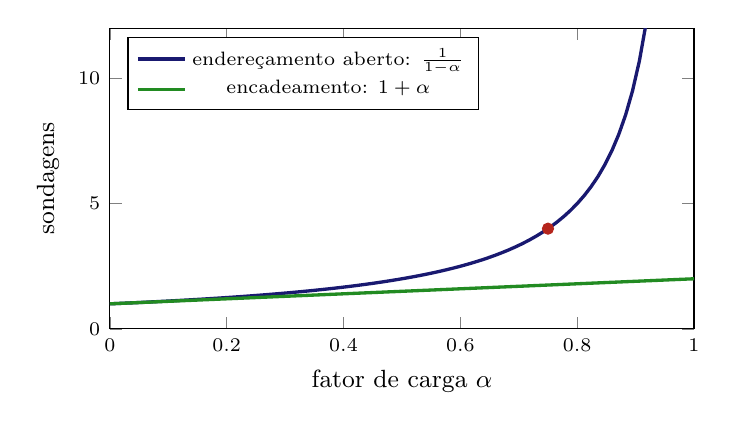
\begin{tikzpicture}
\begin{axis}[width=9cm, height=5.4cm, xmin=0, xmax=1, ymin=0, ymax=12, xlabel={fator de carga $\alpha$}, ylabel={sondagens}, tick label style={font=\scriptsize}, label style={font=\small},
  legend style={font=\scriptsize, at={(0.03,0.97)}, anchor=north west}]
\addplot[very thick, MidnightBlue, domain=0:0.93, samples=80] {1/(1-x)};
\addplot[very thick, ForestGreen, domain=0:1] {1+x};
\addplot[only marks, mark=*, BrickRed] coordinates {(0.75,4)};
\legend{endereçamento aberto: $\frac1{1-\alpha}$, encadeamento: $1+\alpha$}
\end{axis}
\end{tikzpicture}
\end{figura}

\begin{exemplo}[Dimensionando a tabela]
Uma tabela com encadeamento e $m=800$ posições guarda $n=600$ chaves: $\alpha=0{,}75$, e cada lista tem, em média, menos de uma chave; uma busca sem sucesso examina, em média, 0,75 chave depois de calcular o hash. Se as mesmas 600 chaves estivessem numa tabela com endereçamento aberto de 800 posições, uma busca sem sucesso faria em média até $\frac1{1-0{,}75}=4$ sondagens; com só 650 posições ($\alpha\approx0{,}92$), seriam até cerca de 13. Por isso, no endereçamento aberto, a tabela é redimensionada bem antes de encher.
\end{exemplo}

\begin{roteiro}[Tabela hash ou árvore de busca?]
Use uma \textbf{tabela hash} quando só forem necessárias inserção, busca e remoção por chave exata e o desempenho médio importar mais que a garantia de pior caso. Use uma \textbf{árvore balanceada} (AVL ou rubro-negra) quando for preciso manter a ordem das chaves --- mínimo, máximo, sucessor, percurso em ordem, consultas por intervalo --- ou quando for exigida uma garantia de $O(\log n)$ no pior caso.
\end{roteiro}

\begin{cuidado}[Armadilhas das tabelas hash]
\begin{itemize}
  \item Esperar $O(1)$ no pior caso: o tempo constante é \emph{esperado}, sob a hipótese de uma boa função hash; com chaves escolhidas por um adversário e uma função fixa, tudo pode cair no mesmo endereço.
  \item Usar uma função que ignora parte da chave (por exemplo, só os primeiros caracteres de strings longas e parecidas): as colisões se multiplicam.
  \item Deixar a tabela de endereçamento aberto encher: o custo cresce como $\frac1{1-\alpha}$, e com $\alpha=1$ não há onde inserir.
  \item Remover no endereçamento aberto esvaziando a posição, em vez de marcá-la como ``removida''.
\end{itemize}
\end{cuidado}

\begin{chave}
Função hash: chave $\to$ endereço. Colisões são inevitáveis; tratam-se por encadeamento (listas) ou por endereçamento aberto (sondagem linear, quadrática ou duplo hashing). Com fator de carga $\alpha=O(1)$, as operações custam $O(1)$ esperado; o pior caso é $\Theta(n)$. Tabelas hash não mantêm ordem.
\end{chave}

% ----------------------------------------------------------------
\section{Exercícios}
\excurso
\begin{exercicio}{hs-pesq}[Pesquisa]
Disserte sobre: a definição e a motivação das tabelas hash; definição e exemplos de funções de dispersão clássicas; o problema das colisões; o tratamento de colisões por encadeamento exterior e interior e por endereçamento aberto; e a complexidade de pior caso da busca por uma chave.
\end{exercicio}

\excompl
\begin{exercicio}{hs-abertos}[Complementar]
Insira as chaves $10,22,31,4,15,28,17,88,59$, nessa ordem, numa tabela de tamanho $m=11$ com $h(k)=k\bmod11$, usando (a) sondagem linear; (b) sondagem quadrática com $h(k,i)=(h(k)+i+3i^2)\bmod11$; (c) duplo hashing com $h_2(k)=1+(k\bmod10)$.
\end{exercicio}
\begin{exercicio}{hs-encad}[Complementar]
Insira $5,28,19,15,20,33,12,17,10$ numa tabela com encadeamento exterior, $m=9$ e $h(k)=k\bmod9$. Qual o tamanho da maior lista?
\end{exercicio}
\begin{exercicio}{hs-primo}[Complementar]
Por que, no método da divisão, convém escolher $m$ primo e longe de potências de 2? Dê um exemplo do que dá errado com $m=2^r$.
\end{exercicio}
\begin{exercicio}{hs-remove}[Complementar]
No endereçamento aberto, por que a remoção não pode simplesmente esvaziar a posição? Como contornar o problema?
\end{exercicio}
\begin{exercicio}{hs-carga}[Complementar]
Uma tabela com encadeamento tem $m=500$ posições e guarda $n=1000$ chaves. Qual o fator de carga e o comprimento médio das listas? Quantas comparações, em média, faz uma busca sem sucesso?
\end{exercicio}
\begin{exercicio}{hs-sondagens}[Complementar]
Com endereçamento aberto e hashing uniforme, quantas sondagens, em média, faz uma busca sem sucesso quando a tabela está com fator de carga $0{,}5$? E com $0{,}9$? O que isso sugere sobre quando redimensionar a tabela?
\end{exercicio}
\begin{exercicio}{hs-mult}[Complementar]
Calcule $h(k)=\floor{m\,(kA\bmod1)}$ com $m=1000$, $A=(\sqrt5-1)/2\approx0{,}6180339887$, para $k=123456$ e $k=123457$.
\end{exercicio}
\begin{exercicio}{hs-universal}[Complementar]
O que é uma família universal de funções hash? Por que sortear a função de uma família universal protege contra entradas escolhidas para causar muitas colisões?
\end{exercicio}
\begin{exercicio}{hs-string}[Complementar]
Escreva o cálculo de $h(s)=\big(\sum_{i=0}^{L-1}s_i\,b^{L-1-i}\big)\bmod m$ pela regra de Horner, sem calcular potências grandes. Por que $b$ e $m$ não devem ter fatores em comum?
\end{exercicio}
\begin{exercicio}{hs-doissoma}[Complementar]
Dado um vetor de $n$ inteiros e um valor $x$, decida em $O(n)$ esperado se há dois elementos com soma $x$.
\end{exercicio}
\begin{exercicio}{hs-repetido}[Complementar]
Encontre, em $O(n)$ esperado, o primeiro elemento que se repete numa sequência de $n$ valores.
\end{exercicio}
\begin{exercicio}{hs-ordem}[Complementar]
Mostre que encontrar o sucessor de uma chave numa tabela hash pode custar $\Theta(n)$, enquanto numa AVL custa $O(\log n)$. Que outras operações têm a mesma limitação?
\end{exercicio}
\begin{exercicio}{hs-rehash}[Complementar]
Uma tabela dobra de tamanho e reinsere todas as chaves sempre que o fator de carga passa de $1/2$. Mostre que cada inserção custa $O(1)$ amortizado.
\end{exercicio}
\begin{exercicio}{hs-agrup}[Complementar]
Explique o agrupamento primário da sondagem linear e por que, quando uma posição fica no fim de um grupo de $k$ posições ocupadas, ela tem probabilidade maior de ser ocupada na próxima inserção.
\end{exercicio}
\begin{exercicio}{hs-duplo}[Complementar]
No duplo hashing, por que $h_2(k)$ precisa ser primo com $m$? O que acontece se $m=10$ e $h_2(k)=5$?
\end{exercicio}
\begin{exercicio}{hs-remencad}[Complementar]
Com encadeamento exterior, como remover uma chave em $O(1)$, dado um ponteiro para o seu nó? Que tipo de lista é necessário?
\end{exercicio}
\begin{exercicio}{hs-perfeito}[Complementar \estrela]
Para um conjunto \emph{fixo} de $n$ chaves, descreva a ideia do \emph{hashing perfeito} em dois níveis, que garante buscas em $O(1)$ no pior caso com memória $O(n)$ esperada.
\end{exercicio}
\begin{exercicio}{hs-distintos}[Complementar]
Conte quantos valores distintos há numa sequência de $n$ inteiros arbitrários, em $O(n)$ esperado. Como fazer em $O(n\log n)$ no pior caso?
\end{exercicio}
\begin{exercicio}{hs-tamanho}[Complementar]
Uma tabela com endereçamento aberto vai guardar $10^6$ chaves, e o fator de carga não deve passar de $0{,}75$. Qual o tamanho mínimo da tabela? Que valor de $m$ você escolheria para usar o método da divisão?
\end{exercicio}
\begin{exercicio}{hs-busca}[Complementar]
Na tabela da Figura~\ref{fig:sondagem} (sondagem linear, $m=13$), quantas sondagens faz uma busca por 31? E uma busca sem sucesso por 57? E por 26? O que esses números mostram sobre o agrupamento?
\end{exercicio}
\begin{exercicio}{hs-reinsere}[Complementar]
Na mesma tabela, remova o 44, marcando a posição como ``removida'', e depois insira o 70, que não está na tabela. Em que posição o 70 fica? Quantas sondagens faz, em seguida, uma busca pelo 32?
\end{exercicio}
\begin{exercicio}{hs-univsim}[Complementar]
Com $p=17$, $m=6$ e a família $h_{a,b}(k)=((ak+b)\bmod17)\bmod6$, calcule os endereços das chaves 3, 8 e 14 para $(a,b)=(2,7)$ e para $(a,b)=(11,3)$. Em qual dos casos há colisão?
\end{exercicio}
\begin{exercicio}{hs-horner}[Complementar]
Com as letras valendo $\mathtt a=1,\dots,\mathtt z=26$, $b=31$ e $m=97$, calcule pela regra de Horner o endereço de ``casa'' e o de ``saca''. As duas palavras têm as mesmas letras: elas colidem? O que aconteceria com uma função que só somasse os valores das letras?
\end{exercicio}
